\msection{Offensive Diversification: Malware evasion}

The primary malicious use of WebAssembly in browsers is cryptojacking \cite{musch2019new}. 
This is due to the essence of cryptojacking, the faster the mining, the better. 
Although the research of Lehmann and colleagues \cite{Hilbig2021AnES} suggests a decline in browser-based cryptominers, mainly due to the shutdown of Coinhive, a 2022 report by Kaspersky indicates that the use of cryptominers is on the rise \cite{kasperksy}. 
This underscores the ongoing need for effective automatic detection of cryptojacking malware.


Both antivirus software and browsers have implemented measures to detect cryptojacking. For instance, Firefox employs deny lists to detect cryptomining activities \cite{firefoxcrypto}. 
The academic community has also contributed to the body of work on detecting or preventing WebAssembly-based cryptojacking, as outlined in \autoref{background:wasm:analysis}. 
However, it's worth noting that malicious actors can employ evasion techniques to circumvent these detection mechanisms. 
Bhansali et al. are among the first who have investigated how WebAssembly cryptojacking could potentially evade detection \cite{10.1145/3507657.3528560}, highlighting the critical importance of this use case. 
For an in-depth discussion on this topic, we direct the reader to our contribution \cite{EVASION}.
The use of case illustrated in the subsequent sections uses Offensive Software Diversification for the sake of evading malware detection in \Wasm. 

\todo{Replace by a time diagram.}

\msubsection{Threat model: cryptojacking}

Let us illustrate the threat model in which a malicious \wasm binary could be involved.
\autoref{fig:attack_crypto} illustrates a browser attack scenario:
a practical WebAssembly cryptojacking attack consists of three components: a WebAssembly binary, a JavaScript wrapper, and a backend cryptominer pool. 
The WebAssembly binary is responsible for executing the hash calculations, which consume significant computational resources. 
The JavaScript wrapper facilitates the communication between the WebAssembly binary and the cryptominer pool.

\begin{figure}[h]
    \centering
    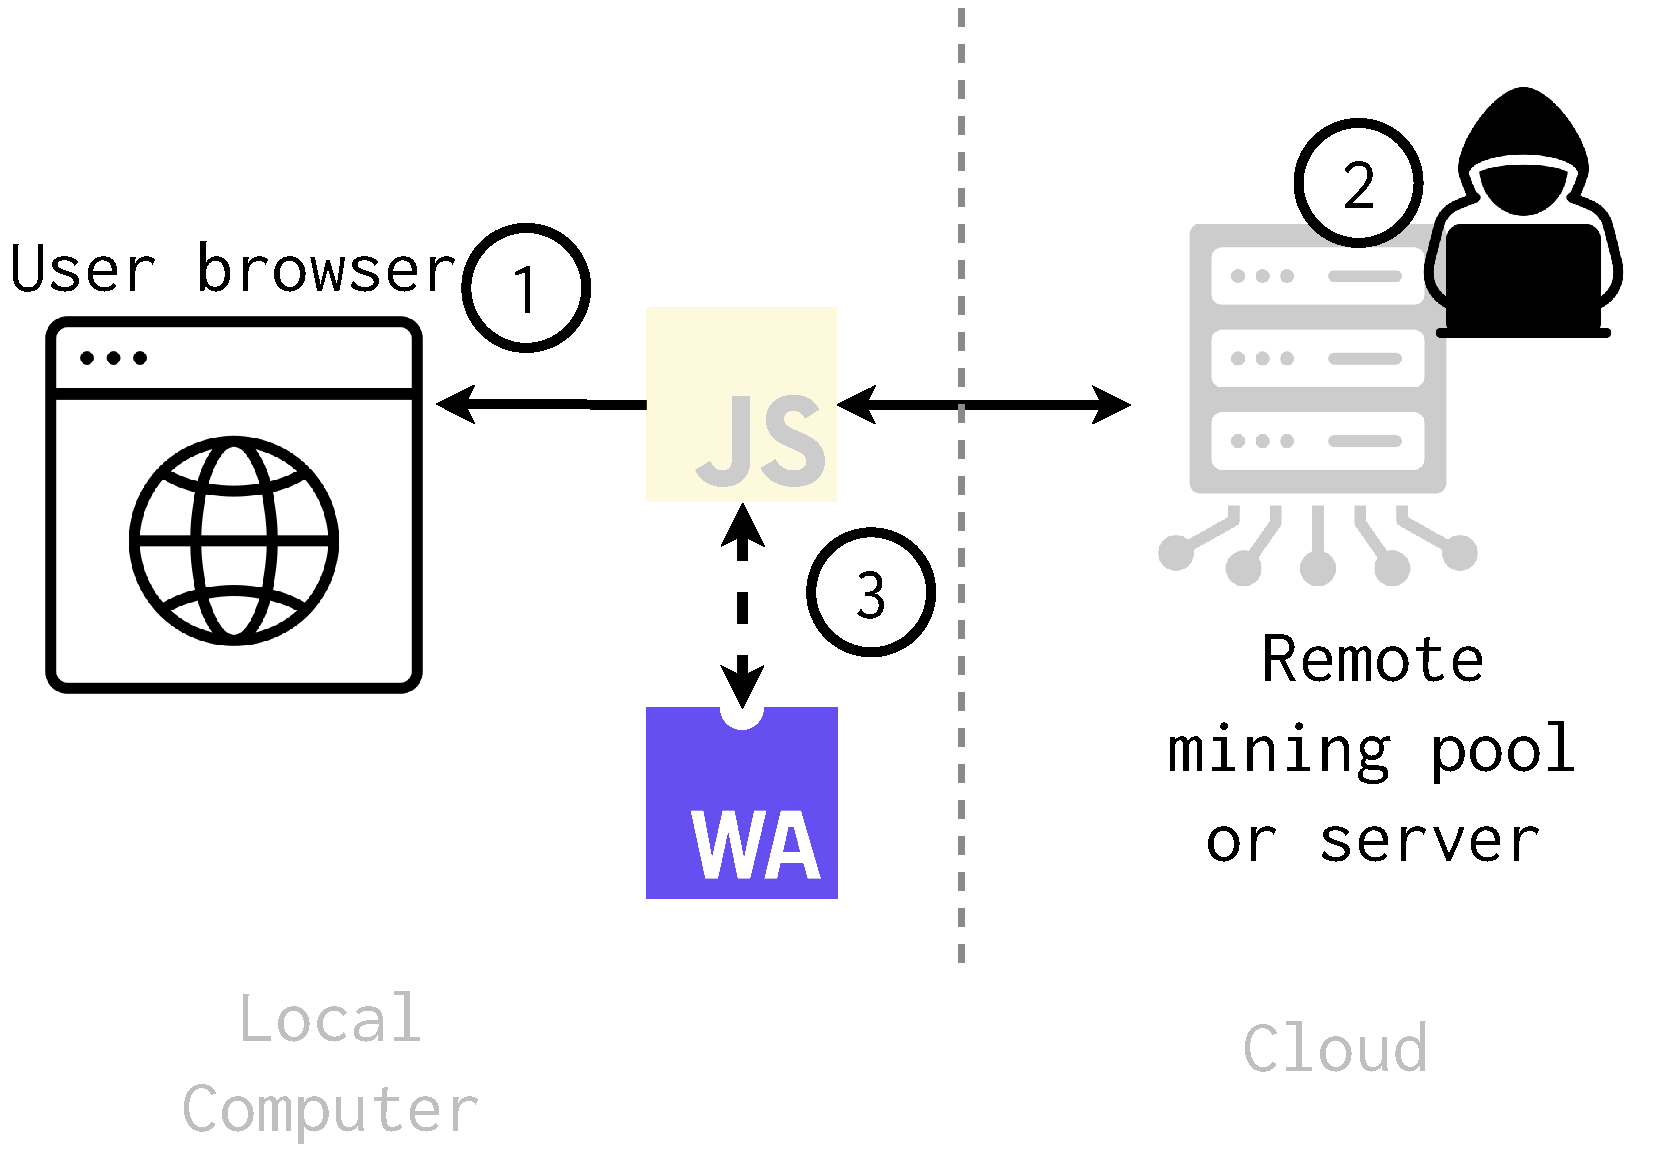
\includegraphics[width=0.6\linewidth]{figures/attack_crypto.pdf}
    \caption{Cryptojacking components.}
    \label{fig:attack_crypto}
\end{figure}

For the previous triad to work, the following steps are executed.
First, the victim visits a web page infected with the cryptojacking code. 
The web page establishes a channel to the cryptominer pool, which then assigns a hashing job to the infected browser. 
The WebAssembly cryptominer calculates thousands of hashes inside the browser. 
Once the malware server receives acceptable hashes, it is rewarded with cryptocurrencies for the mining. 
Then, the server assigns a new job, and the mining process starts over.

\begin{figure}
    \centering
    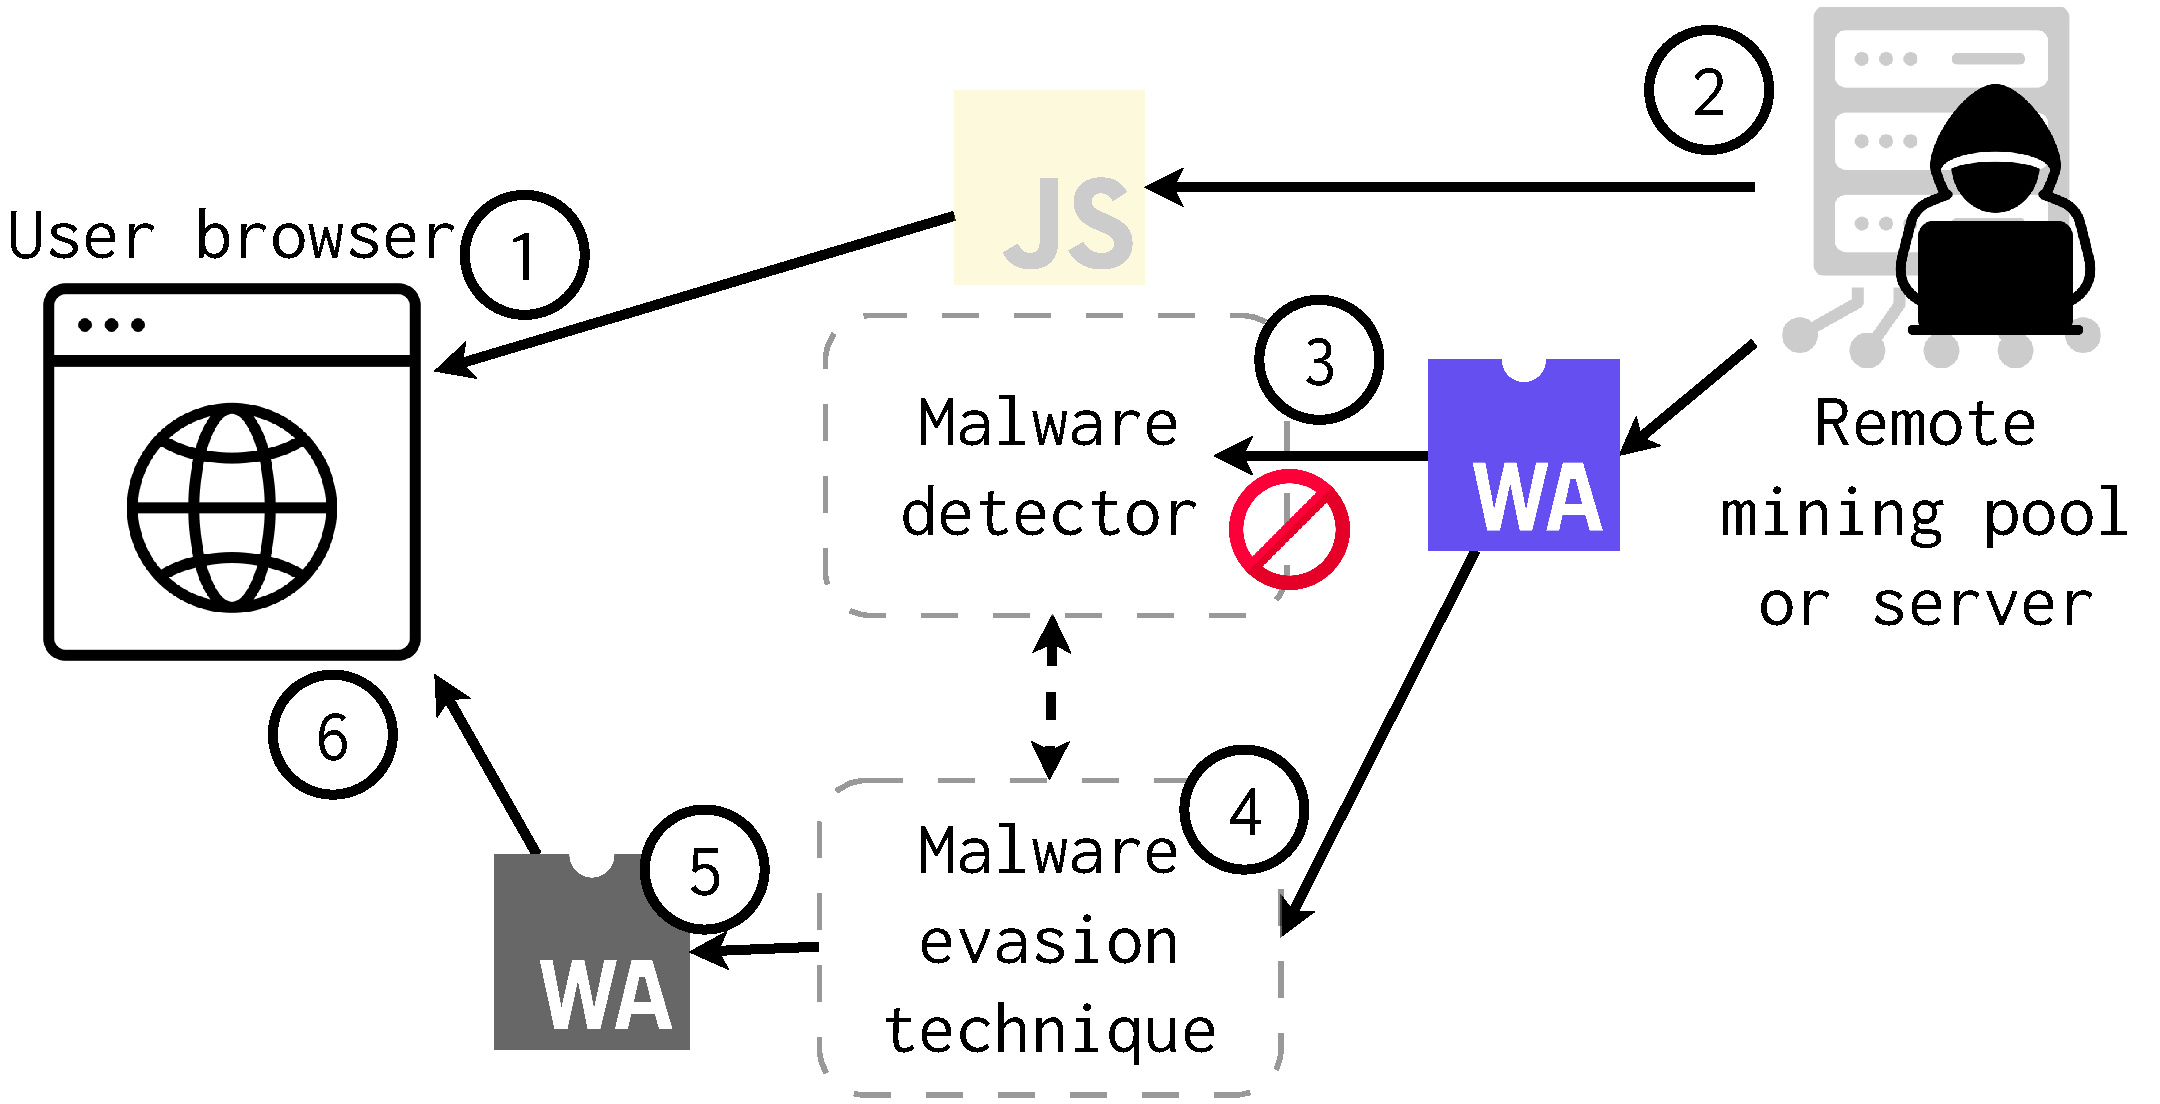
\includegraphics[width=0.4\linewidth]{figures/threat_model.pdf}
    \caption{}
    \label{fig:threat_model}
\end{figure}




\msubsection{Approach}


Several techniques, as outlined in \autoref{background:wasm:analysis}, can be directly implemented in browsers to thwart cryptojacking by identifying the malicious \Wasm components. 
Such defense scenario is illustrated in \autoref{fig:threat_model}, where the \Wasm binary is blocked in \step{3}.
The primary aim of this use of case is to investigate the effectiveness of code diversification as a means to circumvent cryptojacking defenses. 
Specifically, we assess whether the following evasion workflow can successfully bypass existing security measures:

\begin{enumerate}
    
    \item The user lands on a webpage infected with cryptojacking malware, which leverages network resources for execution—corresponding to \step{1} and \step{2} in \autoref{fig:threat_model}. 
    Notice that, various methods can be used to inject cryptojacking malware, including malicious browser extensions, malvertising, compromised websites, or deceptive links \cite{9566204}.
    
    \item A malware detection mechanism identifies and blocks malicious WebAssembly binaries at \step{3}. 
    For example, a network proxy could intercept and forward these resources to an external detection service via its API.
    
    \item Anticipating that a specific malware detection system is consistently used for defense, the attacker swiftly generates a variant of the WebAssembly cryptojacking malware designed to evade detection at \step{4}.
    
    \item The attacker delivers the modified binary instead of the original one \step{5}, which initiates the cryptojacking process and compromises the browser \step{6}. The detection method is completely oblivious to the malicious nature of the binary, and the attack is successful.
    
\end{enumerate}

To empirically validate this evasion scenario, we conducted experiments on 33 cryptojacking malware samples, curated from the 8643 binaries in the wasmbench dataset \cite{Hilbig2021AnES}. 
These 33 binaries were flagged as potentially hazardous by at least one antivirus vendor on VirusTotal. 
We employed WASM-MUTATE to simulate \step{4} in \autoref{fig:threat_model}. 
Our evaluation focuses on three key metrics: the success rate of evading VirusTotal's detection mechanisms across the 33 binaries, the speed at which WASM-MUTATE generates a detection-evasive variant, and the performance impact on the variants that successfully evade the detection.

\todo{Explain binary and numeric oracle here to define the defense system.}

%\lipsum[1]

%\lipsum[1]

\msubsection{Results}


\begin{table}
    \centering
    \begin{tabular}{l l | l l | l l |}
        \hline
        Hash & \#D & \multicolumn{2}{c|}{Uncontrolled diversification} & \multicolumn{2}{c|}{Controlled diversification} \\
        \hline
        &  & Max. #evaded & Mean #trans. & Max. #evaded & Mean #trans. \\
        \hline\hline
        A & 1 & 1 & 1 & 1 \\
    \end{tabular}
    \caption{TODO}
    \label{offensive:results:fast}
\end{table}

\todo{Table: Uncontrolled and controlled diversification}


\todo{How many iterations are needed to evade the detection? Compare with the table in chapter 3, 10000 variants in one hour is equivalent to say that we can evade the detection in 10 minutes.}




\renewcommand\arraystretch{1.2}
\begin{adjustbox}{width=1\linewidth}
\rev{
  \begin{tabular}{c c | cr  cr  cr || cr  cr  cr}

        \toprule
           Hash &  Original h/s & \multicolumn{6}{c||}{Baseline algorithm} & \multicolumn{6}{c}{MCMC algorithm} \\
         \hline


        0d996462  &  116.0     &  100\%  & 25 (0.22)   &  100\%  & 24 (0.21)   &  100\%  & 26 (0.22)    &  100\%  & 116 \textbf{(1.00)}    &  100\%  & 70 (0.60)   &  100\%  & 67 (0.58)  \\ &    &  100\%  & 116 \textbf{(1.00)}    &  100\%  & 110 (0.95)   &  100\%  & 30 (0.26)    &  100\%  & 110 (0.95)   &  100\%  & 76 (0.66)   &  100\%  & 60 (0.52)  \\ &    &  100\%  & 55 (0.47)   &  100\%  & 27 (0.23)   &  100\%  & 23 (0.20)    &  100\%  & 86 (0.74)   &  100\%  & 60 (0.52)   &  100\%  & 72 (0.62)  \\ &    &  100\%  & 27 (0.23)    &   &   &   &   &   100\%  & 76 (0.66)  \\
        \hline
 a32a6f4b  &  48.0   &   100\%  & 25 (0.52)   &  100\%  & 24 (0.50)   &  100\%  & 24 (0.50)    &  100\%  & 26 (0.54)   &  100\%  & 45 (0.94)   &  100\%  & 41 (0.85)  \\ &    &  100\%  & 26 (0.54)   &  100\%  & 25 (0.52)   &  100\%  & 26 (0.54)    &  100\%  & 46 (0.96)   &  100\%  & 41 (0.85)   &  100\%  & 45 (0.94)  \\ &    &  100\%  & 26 (0.54)   &  100\%  & 24 (0.50)   &  100\%  & 25 (0.52)    &  100\%  & 44 (0.92)   &  100\%  & 42 (0.88)   &  100\%  & 45 (0.94)  \\ &    &  100\%  & 23 (0.48)    &   &  &  &  &  100\%  & 45 (0.94)  \\
        \hline
 fbdd1efa  &  37.0     &  100\%  & 25 (0.68)   &  100\%  & 25 (0.68)   &  100\%  & 25 (0.68)    &  100\%  & 28 (0.76)   &  100\%  & 47 \textbf{(1.27)}    &  100\%  & 48 \textbf{(1.30)}   \\ &    &  100\%  & 25 (0.68)   &  100\%  & 26 (0.70)   &  100\%  & 26 (0.70)    &  100\%  & 47 \textbf{(1.27)}    &  100\%  & 47 \textbf{(1.27)}    &  100\%  & 53 \textbf{(1.43)}   \\ &    &  100\%  & 25 (0.68)   &  100\%  & 25 (0.68)   &  100\%  & 25 (0.68)    &  100\%  & 48 \textbf{(1.30)}    &  100\%  & 48 \textbf{(1.30)}    &  100\%  & 49 \textbf{(1.32)}   \\ &    &  100\%  & 25 (0.68)     &   &  &  &   &  100\%  & 47 \textbf{(1.27)}   \\
        \hline
   d2141ff2  &  113.0    &  100\%  & 54 (0.48)   &  100\%  & 55 (0.49)   &  100\%  & 55 (0.49)    &  100\%  & 107 (0.95)   &  100\%  & 107 (0.95)   &  100\%  & 107 (0.95)  \\ &    &  100\%  & 57 (0.50)   &  100\%  & 56 (0.50)   &  100\%  & 56 (0.50)    &  100\%  & 109 (0.96)   &  100\%  & 106 (0.94)   &  100\%  & 100 (0.88)  \\ &    &  100\%  & 57 (0.50)   &  100\%  & 53 (0.47)   &  100\%  & 53 (0.47)    &  100\%  & 101 (0.89)   &  100\%  & 100 (0.88)   &  100\%  & 107 (0.95)  \\ &    &  100\%  & 55 (0.49)     &   &  &  &   &  100\%  & 107 (0.95)  \\
        \hline
   046dc081  &  118.0    &  100\%  & 58 (0.49)   &  100\%  & 60 (0.51)   &  100\%  & 59 (0.50)    &  100\%  & 118 \textbf{(1.00)}    &  100\%  & 120 \textbf{(1.02)}    &  100\%  & 119 \textbf{(1.01)}   \\ &    &  100\%  & 60 (0.51)   &  100\%  & 55 (0.47)   &  100\%  & 62 (0.53)    &  100\%  & 120 \textbf{(1.02)}    &  100\%  & 116 (0.98)   &  100\%  & 120 \textbf{(1.02)}   \\ &    &  100\%  & 55 (0.47)   &  100\%  & 50 (0.42)   &  100\%  & 57 (0.48)    &  100\%  & 119 \textbf{(1.01)}    &  100\%  & 120 \textbf{(1.02)}    &  100\%  & 119 \textbf{(1.01)}   \\ &    &  100\%  & 55 (0.47)     &   &  &  &   &  100\%  & 120 \textbf{(1.02)}   \\
        \hline
   006b2fb6  &  8.0    &  100\%  & 7 (0.88)   &  100\%  & 6 (0.75)   &  100\%  & 4 (0.50)    &  100\%  & 6 (0.75)   &  100\%  & 6 (0.75)   &  100\%  & 6 (0.75)  \\ &    &  100\%  & 9 \textbf{(1.12)}    &  100\%  & 6 (0.75)   &  100\%  & 4 (0.50)    &  100\%  & 6 (0.75)   &  100\%  & 6 (0.75)   &  100\%  & 6 (0.75)  \\ &    &  100\%  & 4 (0.50)   &  100\%  & 6 (0.75)   &  100\%  & 4 (0.50)    &  100\%  & 8 \textbf{(1.00)}    &  100\%  & 9 \textbf{(1.12)}    &  100\%  & 6 (0.75)  \\ &    &  100\%  & 6 (0.75)     &   &  &  &  &  100\%  & 6 (0.75)  \\
        \hline
    
        
    \end{tabular}
}
\end{adjustbox}


\todo{Talk about performance. Highlight the presence of bloating...the faster you compile, the faster you start ahasing. Link this with the paper that Marin shared lately, highlighting the lack of optimization.}




Remarkably, we find 30 cryptominers for which our technique successfully generates variants that evade VirusTotal.
Our set of malware includes 6 cryptojacking programs that are fully reproducible in a controlled environment. 
With them, we assess that our evasion method does not affect malware correctness and generates fully functional malware variants with minimal overhead.

Our work provides evidence that the malware detection community has opportunities to strengthen the automatic detection of cryptojacking WebAssembly malware. 
The results of this work are actionable, as we provide quantitative evidence on specific malware transformations on which detection methods can focus.


\begin{tcolorbox}[title=Contribution paper,boxrule=1pt,arc=.2em,boxsep=1.0mm]
    The case discussed in this section is fully detailed in Cabrera-Arteaga \etal "WebAssembly Diversification for Malware Evasion"
    \emph{at Computers \& Security, 2023}
    \url{https://www.sciencedirect.com/science/article/pii/S0167404823002067}. 
\end{tcolorbox}
